\documentclass[12pt,reqno]{amsart}
\usepackage{/Users/johnmyers/GoogleDrive/tex/handout,/Users/johnmyers/GoogleDrive/tex/customcommands,polynom}
\usepackage{caption}

\hdr{MAT 240}{\S14.1 The partial derivative}

\begin{document}

\textbf{Suggested problems:} 1-13 odd, 17-29 odd

\bigskip
\hrule

\bigskip

\prob The price $P$ in dollars to purchase a used car is a function of its original cost, $C$, in dollars, and its age, $A$, in years.

\medskip
\begin{enumerate}
\item What are the units of $\bd P /\bd A$?

\bigskip
\textcolor{red}{The units are dollar per year.}
\bigskip

\item What is the sign of $\bd P/\bd A$ and why?

\bigskip
\textcolor{red}{The sign should be negative. This is because as a car ages, its value goes down.}
\bigskip

\item What are the units of $\bd P / \bd C$?

\bigskip
\textcolor{red}{The units are dollar per dollar.}
\bigskip

\item What is the sign of $\bd P/\bd C$ and why?

\bigskip
\textcolor{red}{The sign should be positive. This is because a car with a higher original cost should be more expensive to buy used than a car with a cheaper original cost of the same age.}
\bigskip
\end{enumerate}

\prob The figure below shows the surface $z=f(x,y)$. What is the sign of $f_x(0,5)$? What is the sign of $f_y(0,5)$? \textcolor{red}{We have $f_x(0,5)<0$ and $f_y(0,5)>0$.}

\medskip
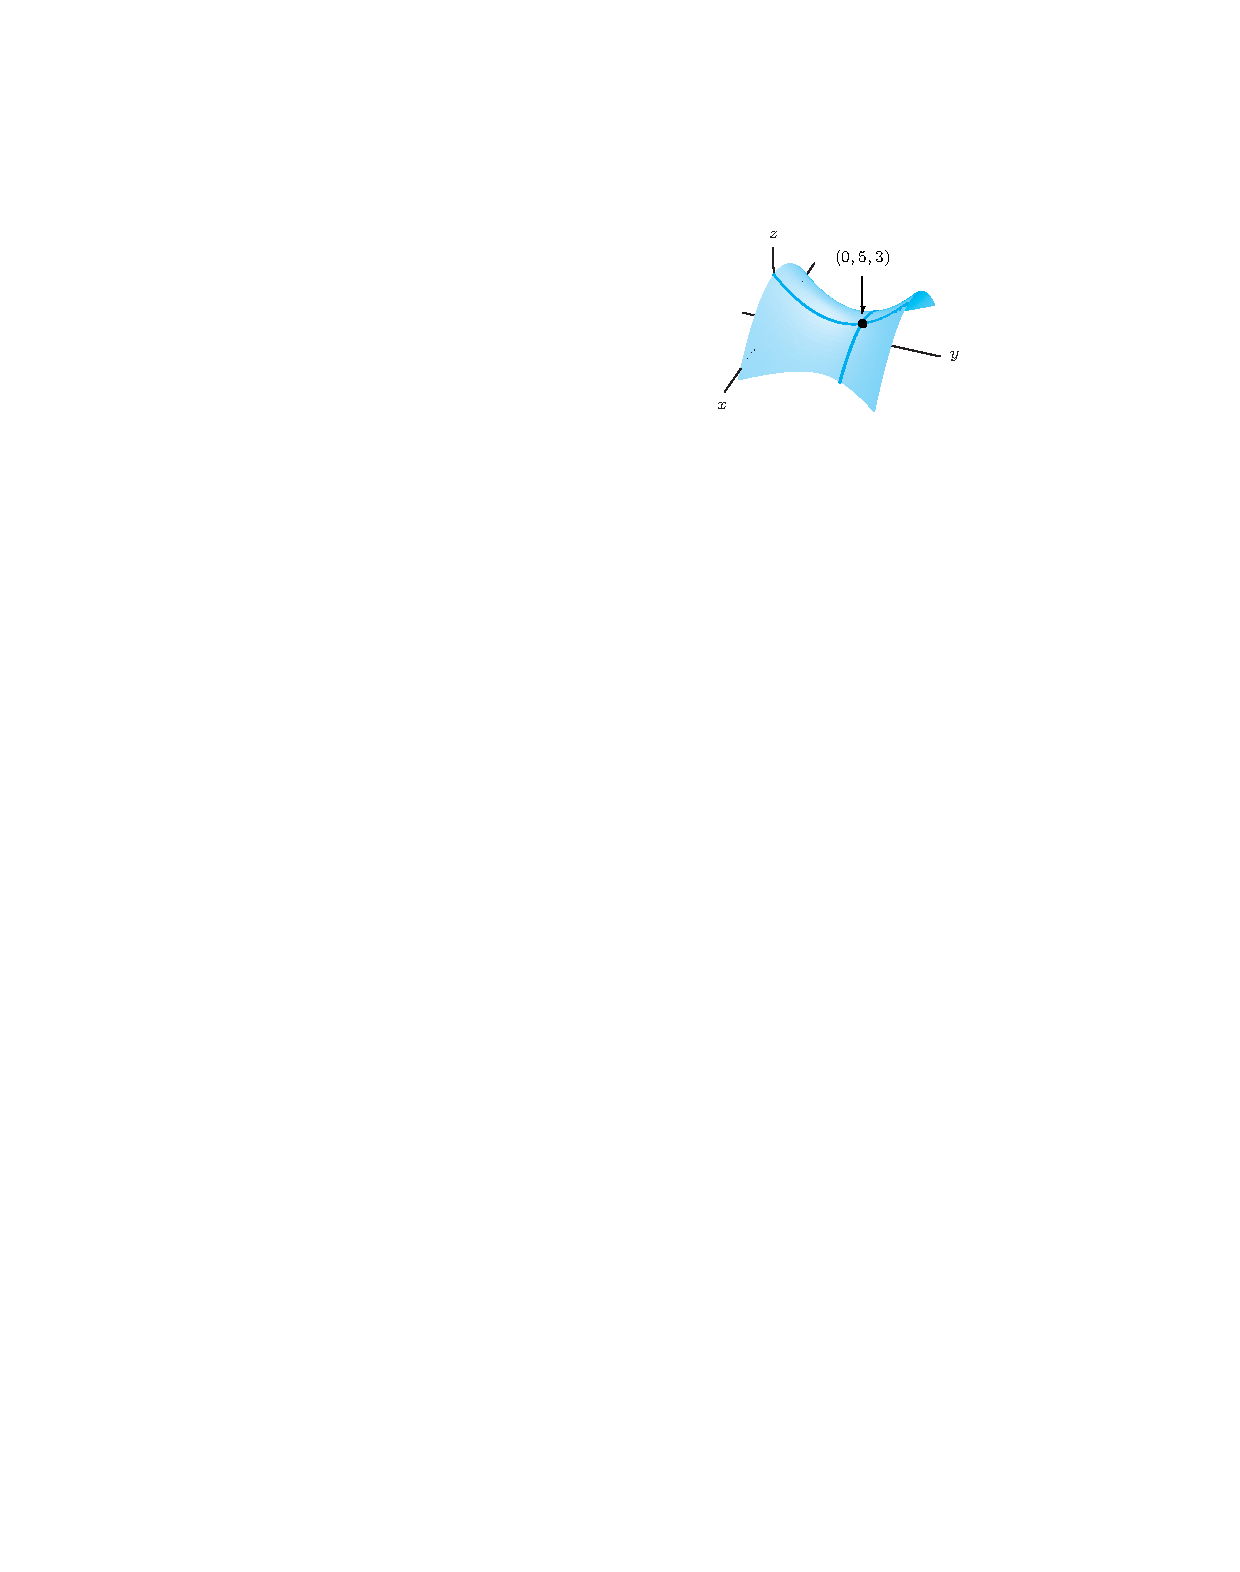
\includegraphics[scale=1.5]{pic4.pdf}

\prob The figure below shows the graph of a function $x=f(x,y)$ on the domain $0\leq x \leq 4$ and $0 \leq y \leq 4$. Use the graph to rank the following quantities in order from smallest to largest: $f_x(3,2)$, $f_x(1,2)$, $f_y(3,2)$, $f_y(1,2)$, $0$. \textcolor{red}{$f_x(1,2) < f_x(3,2) < 0 < f_y(3,2) < f_y(1,2) $}

\medskip
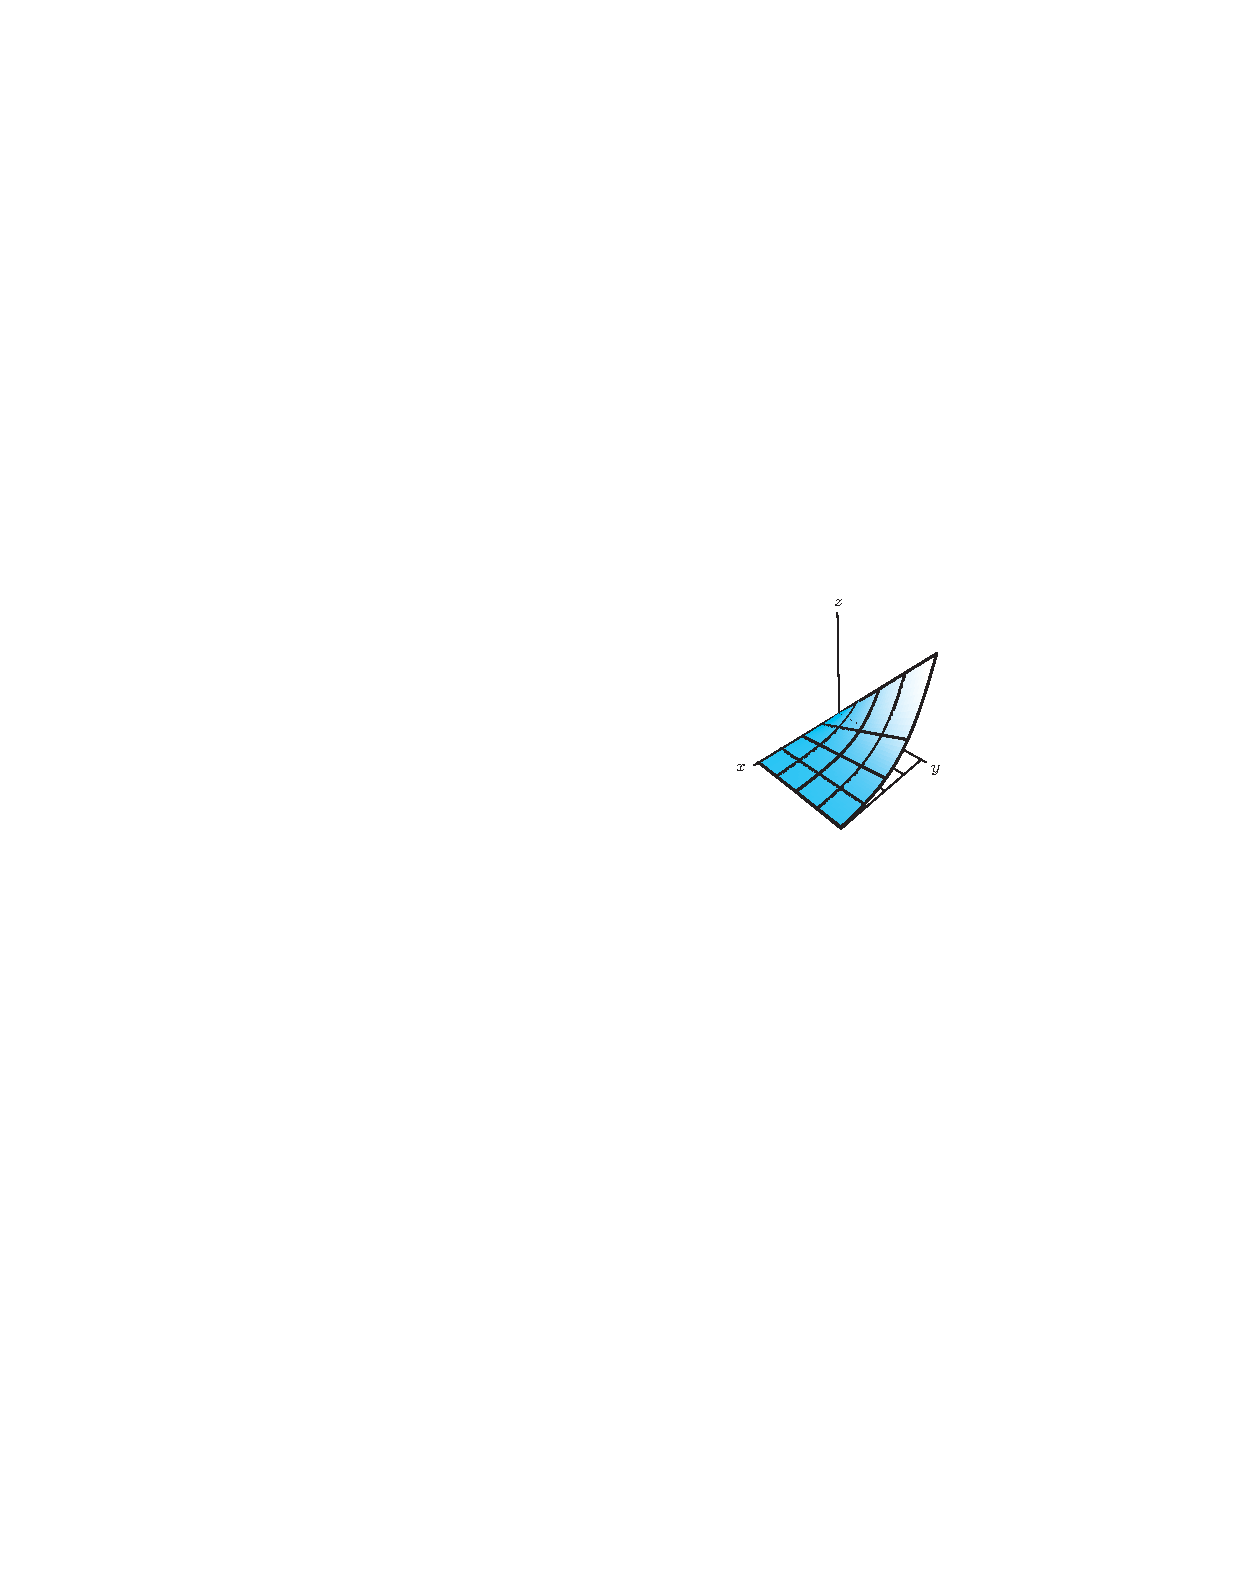
\includegraphics[scale=1.5]{pic3.pdf}

\prob Suppose we are given the contour diagram below of a function $z=f(x,y)$. Is $f_x$ positive or negative? How about $f_y$? \textcolor{red}{$f_x>0$ and $f_y<0$.}

\medskip
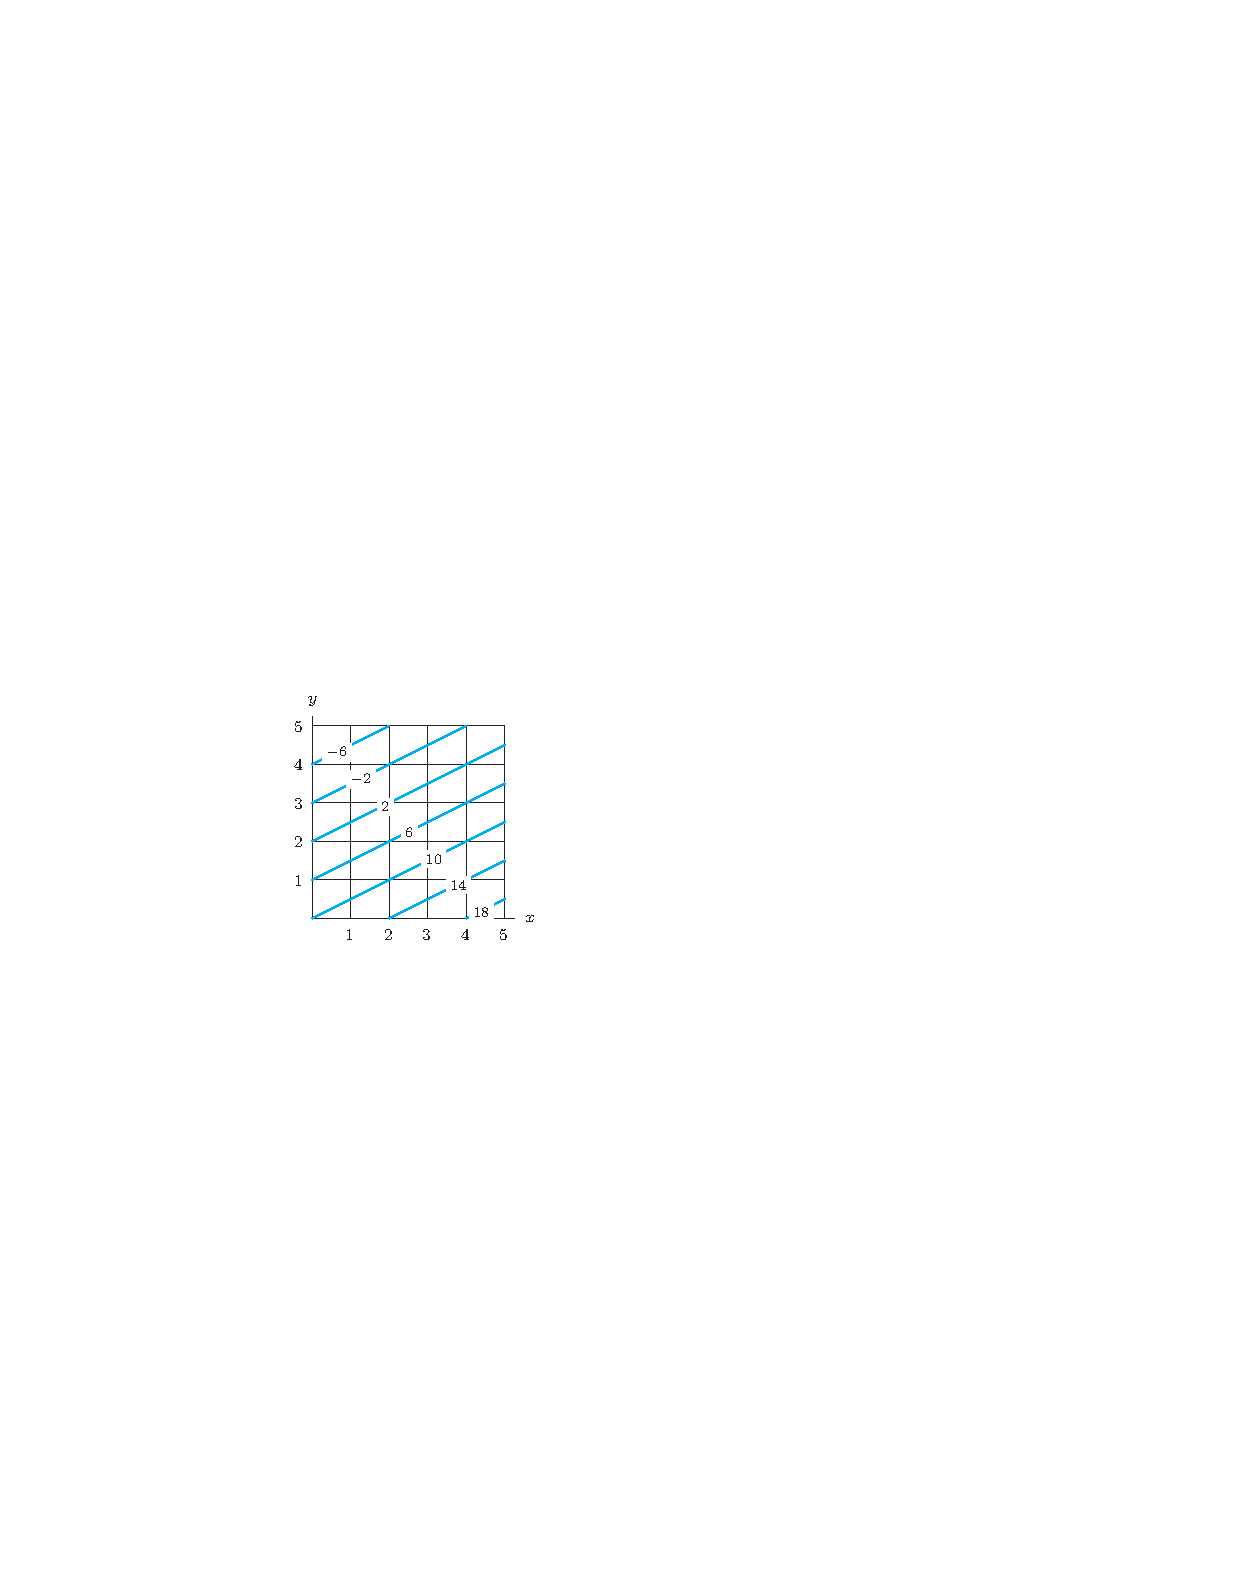
\includegraphics[scale=1.5]{pic1.pdf}

\prob The graph of $z = f (x, y)$ is shown in the figure below. The points $A$ and $B$ are in the $xy$-plane.

\begin{minipage}{0.5\textwidth}
\begin{enumerate}
\item What is the sign of $f_x(A)$? What is the sign of $f_y(A)$?\vspace{1in}
\item The point $P$ in the $xy$-plane moves along a straight line from $A$ to $B$. How does the sign of $f_x(P)$
change? How does the sign of $f_y (P )$ change?
\end{enumerate}
\end{minipage}%
%
\begin{minipage}{0.5\textwidth}
\begin{center}

\includegraphics[scale=1.5]{1.pdf}
\end{center}
\end{minipage}

\bigskip
\textcolor{red}{(a) $f_x(A)>0$ and $f_y(A)<0$. (b) The sign of $f_x(P)$ appears to be positive until the point $P$ crosses the $y$-axis, and then it turns negative. The sign of $f_y(P)$ appears to be negative at all times as $P$ moves from $A$ to $B$.}

\end{document}